\documentclass[12pt,letterpaper]{article}
\usepackage{graphicx,textcomp}
\usepackage{natbib}
\usepackage{setspace}
\usepackage{fullpage}
\usepackage{color}
\usepackage[reqno]{amsmath}
\usepackage{amsthm}
\usepackage{fancyvrb}
\usepackage{amssymb,enumerate}
\usepackage[all]{xy}
\usepackage{endnotes}
\usepackage{lscape}
\newtheorem{com}{Comment}
\usepackage{float}
\usepackage{hyperref}
\newtheorem{lem} {Lemma}
\newtheorem{prop}{Proposition}
\newtheorem{thm}{Theorem}
\newtheorem{defn}{Definition}
\newtheorem{cor}{Corollary}
\newtheorem{obs}{Observation}
\usepackage[compact]{titlesec}
\usepackage{dcolumn}
\usepackage{tikz}
\usetikzlibrary{arrows}
\usepackage{multirow}
\usepackage{xcolor}
\newcolumntype{.}{D{.}{.}{-1}}
\newcolumntype{d}[1]{D{.}{.}{#1}}
\definecolor{light-gray}{gray}{0.65}
\usepackage{url}
\usepackage{listings}
\usepackage{color}

\definecolor{codegreen}{rgb}{0,0.6,0}
\definecolor{codegray}{rgb}{0.5,0.5,0.5}
\definecolor{codepurple}{rgb}{0.58,0,0.82}
\definecolor{backcolour}{rgb}{0.95,0.95,0.92}

\lstdefinestyle{mystyle}{
	backgroundcolor=\color{backcolour},   
	commentstyle=\color{codegreen},
	keywordstyle=\color{magenta},
	numberstyle=\tiny\color{codegray},
	stringstyle=\color{codepurple},
	basicstyle=\footnotesize,
	breakatwhitespace=false,         
	breaklines=true,                 
	captionpos=b,                    
	keepspaces=true,                 
	numbers=left,                    
	numbersep=5pt,                  
	showspaces=false,                
	showstringspaces=false,
	showtabs=false,                  
	tabsize=2
}
\lstset{style=mystyle}
\newcommand{\Sref}[1]{Section~\ref{#1}}
\newtheorem{hyp}{Hypothesis}

\title{Problem Set 2}
\date{Due: February 4, 2026}
\author{Data Visualisation for Social Scientists}

\begin{document}
	\maketitle
	
	\section*{Instructions}
	\begin{itemize}
	\item Please show your work! You may lose points by simply writing in the answer. If the problem requires you to execute commands in \texttt{R}, please include the code you used to get your answers. Please also include the \texttt{.R} file that contains your code. If you are not sure if work needs to be shown for a particular problem, please ask.
\item Your homework should be submitted electronically on GitHub.
\item This problem set is due before 23:59 on Wednesday February 4, 2026. No late assignments will be accepted.
	\end{itemize}
	
	\vspace{.25cm}
	\section*{Study of Religious Congregations in Switzerland}
	
The data for this problem set come from the	National Congregations Study Switzerland (NCSS), which was conducted in 2008–2009 and 2022–2023. The data provide information on organisational structure, staffing, finances, worship practices, youth and educational activities, social composition, external engagement, and inclusion norms. The data were collected using stratified random samples of congregations drawn from comprehensive censuses, with interviews completed by a single knowledgeable key informant in each congregation, most often the spiritual leader.

\subsection*{Data Manipulation}

\begin{enumerate}
\item Load the NCSS .csv file from \href{https://raw.githubusercontent.com/ASDS-TCD/DataViz_2026/refs/heads/main/datasets/NCSS_v1.csv}{GitHub} into your global environment. Use the select() function to keep these variables in your dataframe:
\begin{itemize}
	\item Congregation ID (\texttt{CASEID})
	\item Year (\texttt{YEAR})
	\item Region (\texttt{GDREGION})
	\item Number of official members (\texttt{NUMOFFMBR})
	\item 6-level religious classification (\texttt{TRAD6})
	\item 12-level religious classification (\texttt{TRAD12})
	\item Total income in last fiscal year (\texttt{INCOME})
\end{itemize}
\lstinputlisting[language=R, firstline=12, lastline=23]{PS02_CK.R}  
\begin{description}
	\item In this code, I took the csv file and uploaded it into my R file. From there I selected the variables using the select function, so that my dataframe has only the variables of interest listed above. 
\end{description}
\item Filter the dataset so that you only include Christian, Jewish, and Muslim congregations (Chrétiennes, Juives, Musulmanes) using the \texttt{TRAD6} variable.
\lstinputlisting[language=R, firstline=26, lastline=26]{PS02_CK.R}  
\begin{description}
	\item For filtering the dataset to include only these three congregations, I used the filter function, selected the data and the variable. Then, I used the operator to state that within the variable for TRAD6, I wanted just these values to be present in the dataframe. Note that my R code does have the proper accents for selecting the Christian congregations, but the tex file is having a hard time inserting them. 
\end{description}
\item Compute for the number of congregations by religious classification (\texttt{TRAD6}) in each year, as well as the mean and median total income in last fiscal year (\texttt{INCOME}) by religious classification and year.
\lstinputlisting[language=R, firstline=29, lastline=37]{PS02_CK.R}  
\begin{description}
	\item For this part, I created a new dataset named the cong summary to summarize the mean income, median income, and total value for each of the specifed TRAD6 classifications. The data was grouped by year and TRAD6, then using the summarize function, I calculated the mean, median, and total. In the end I dropped the grouping from the data so I could continue using different grouping practices throughout the assignment. 
\end{description}
\item Create a categorical variable for called \texttt{AVG\_INCOME} that is binary in which 1 = "Above average or average income" and 0 = "Below average income", which indicates if a congregation is $\geq$ average income or $<$ average income among congregations that year.
\lstinputlisting[language=R, firstline=40, lastline=50]{PS02_CK.R}  
\begin{description}
	\item Lastly, I needed to add a new categorical variable for the data frame. To do so, I grouped the data by year and TRAD6 then used the mutate function to add a column for the mean income of these congregations. Then using the case when function, I established the rules for the categorical variable. The code states that when a mean income is over the average it is assigned the value of one and when it is below then it is assigned the value of zero. Also, if the information wasn't given for the icome of the congregation, therefore the mean couldn't be produced, the column was given an NA. 
\end{description}
\end{enumerate}

\subsection*{Data Visualization}

\begin{enumerate}
	\item Create a bar plot visualizing the proportion of congregations above and below the average income (\texttt{AVG\_INCOME}) in each year by 12-level religious classification (\texttt{TRAD12}). Hint: Use \texttt{facet()} for \texttt{YEAR}.
	\lstinputlisting[language=R, firstline=55, lastline=77]{PS02_CK.R}  
		\begin{figure}[H]
		\centering
		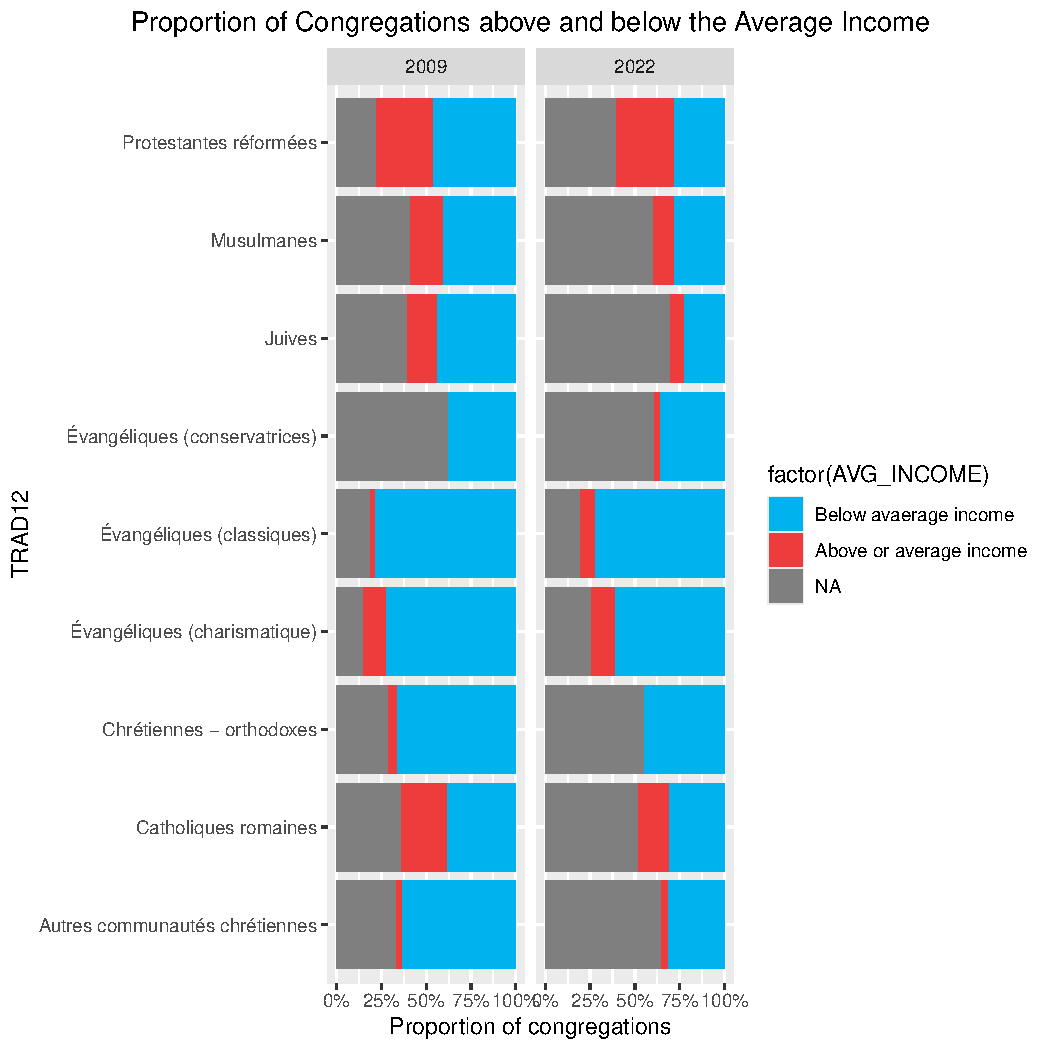
\includegraphics[width=0.7\textwidth]{V1.pdf}
	\end{figure}
	\begin{description}
		\item For this visualization, I classified the data to be used and which variabled that will be choosen for the bar plot. Since the visualization is comparing the TRAD12 classifications, I thought that flipping the coordinates would make each classification easier to read. Using the facet function for the year allowed the visualization to create side by side visualizations for each year in the data (line 13). This allows for side by side comparison of the income levels per classification. 
	\end{description}
	\item Make a histogram using \texttt{geom\_col()} detailing the number of official members using the 12-level religious classification (\texttt{TRAD12}) distinguishing between the 6-level religious classification (\texttt{TRAD6}) in 2022. Hint: Use \texttt{TRAD12} on the x-axis.
		\lstinputlisting[language=R, firstline=80, lastline=94]{PS02_CK.R}  
		\begin{figure}[H]
		\centering
		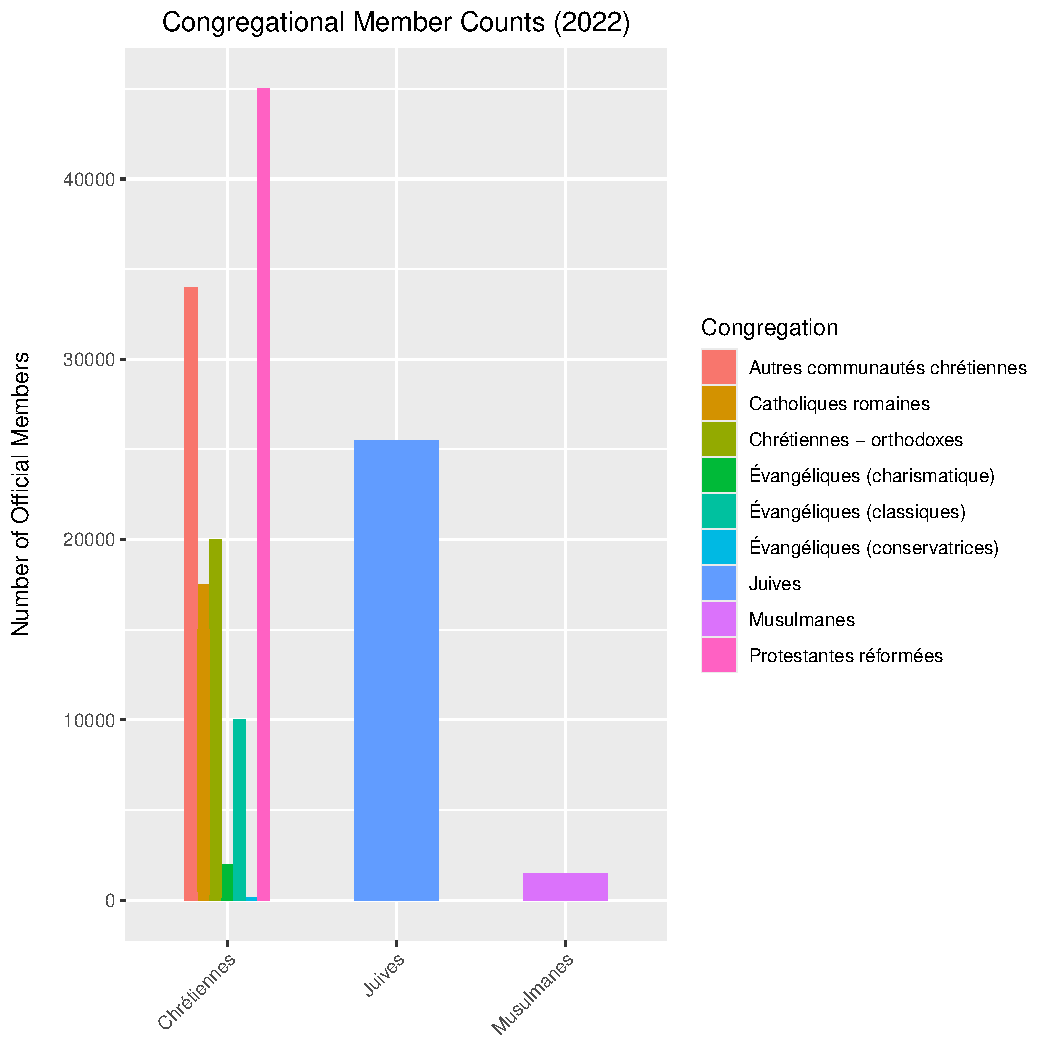
\includegraphics[width=0.7\textwidth]{V2.pdf}
	\end{figure}
	\begin{description}
		\item To start, this visualization asked for the data to be filtered by the year 2022, so I needed to do that as sson as I entered the data into the ggplot function. Then, I used both the TRAD6 and TRAD 12 classifications for the bar plot, which, made for a funky design. Since the Christian group is the only one to have different denominations (TRAD12), the bar graph for that section was broken up. Therefore, you can really see the difference in memember count for each Christian group. I messed arounf with the width of the histogram and the colors (lines 3 and 4) to get a more visually pleasing visualization. I also adjusted the axis titles in lines 5 and 6 so the names of each classification are easy to read. 
			\end{description}
	\item Display the distribution of yearly income (\texttt{INCOME}) in 2022 for congregations in each region (\texttt{GDREGION}) using ridge plots.
	\lstinputlisting[language=R, firstline=97, lastline=115]{PS02_CK.R}  
		\begin{figure}[H]
		\centering
		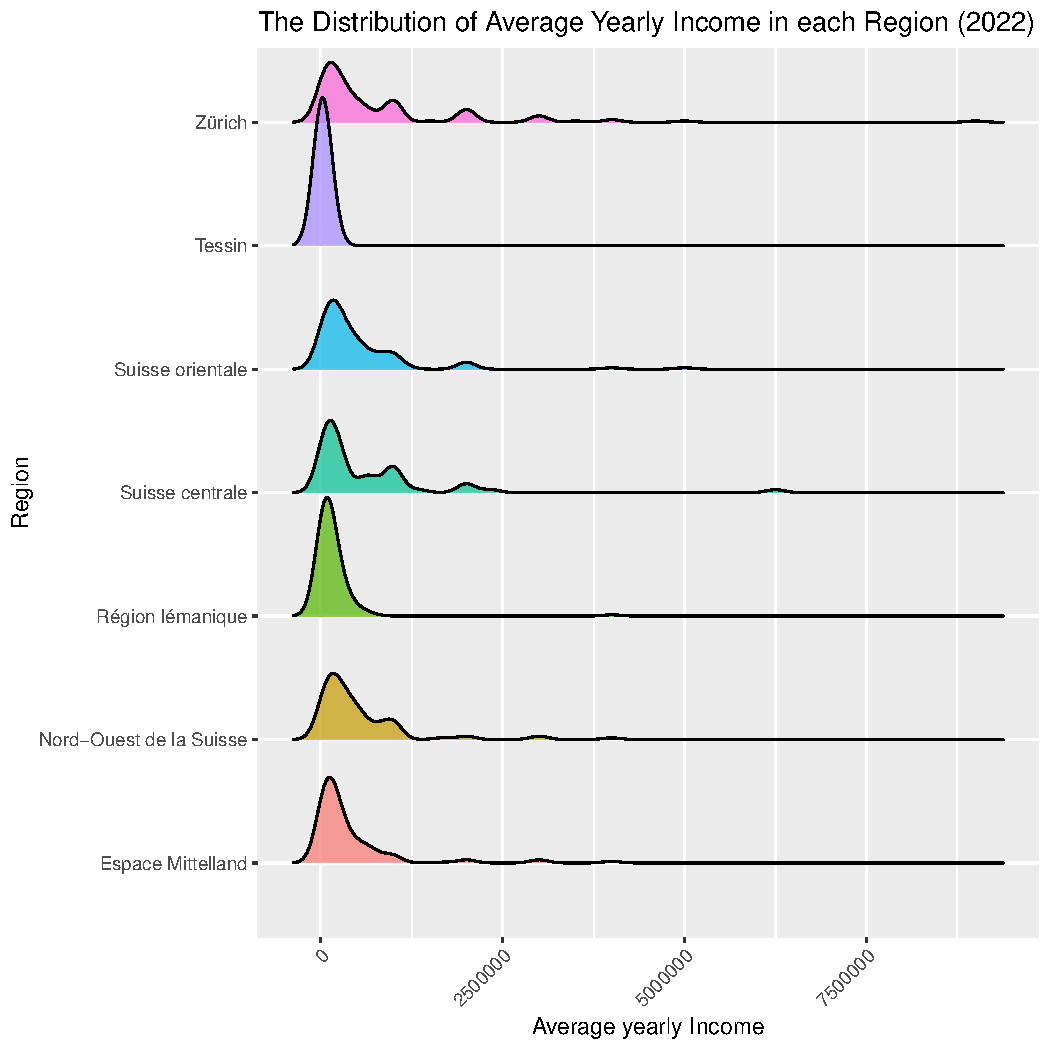
\includegraphics[width=0.7\textwidth]{V3.pdf}
	\end{figure}
	\begin{description}
		\item To start this visualization, I needed to download more packages in order to complete this ridge plot. Once again, I filtered the data by the year 2022 and used income and region as my variables of interest. I filled by region to show the different density distributions for each region in this data frame. I messed around with the x axis (lines 7 and 8) to zoom in on the distributions so that we can see more of the flucuation. By doing so, I found that cutting off the x axis at zero made sense since there is less likely that the year income would be less than zero contextually. 
	\end{description}
	\item Create a boxplot of the number of official members per congregation in 2022 by religious classification (\texttt{TRAD6}) and region (\texttt{GDREGION}). Hint: Use \texttt{facet()} for \texttt{GDREGION}.
	\lstinputlisting[language=R, firstline=118, lastline=134]{PS02_CK.R}  
		\begin{figure}[H]
		\centering
		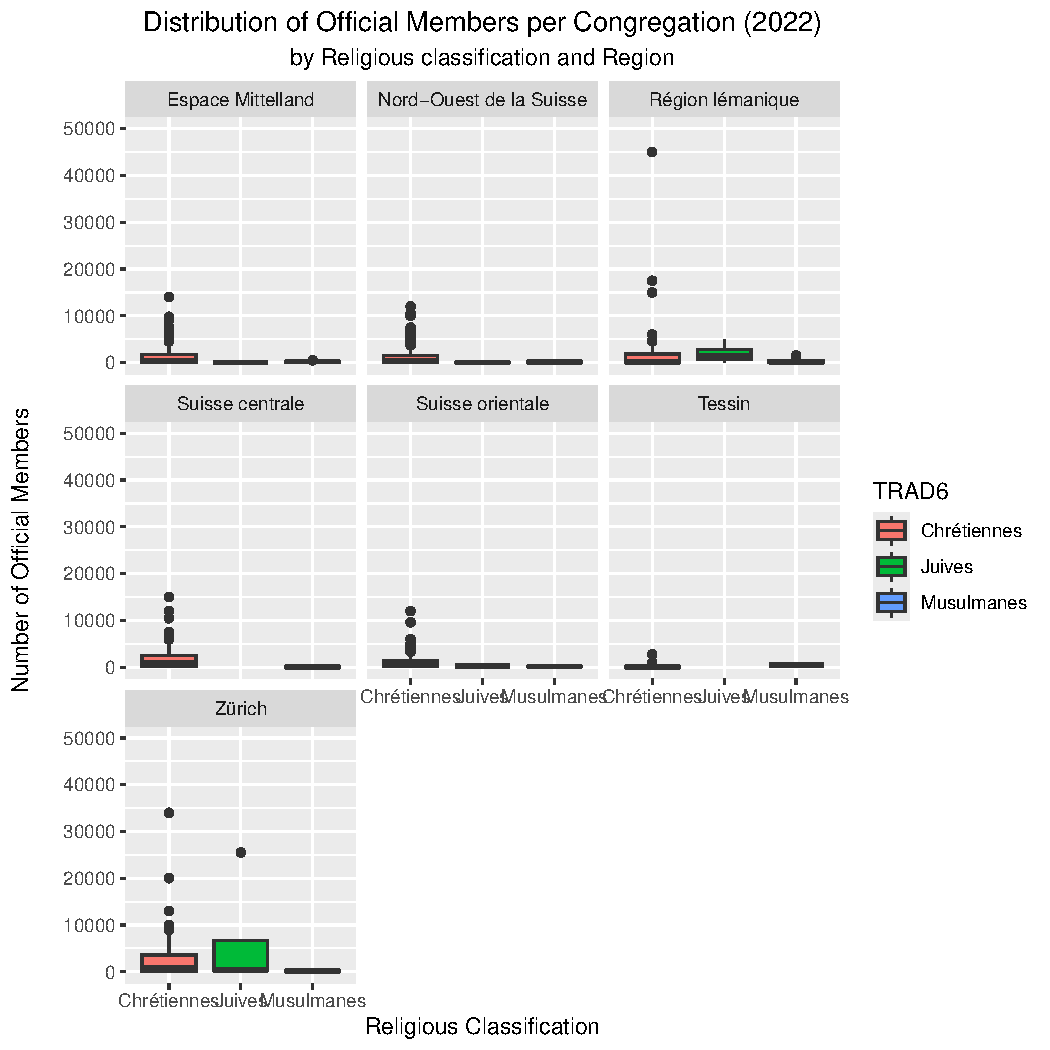
\includegraphics[width=0.7\textwidth]{V4.pdf}
	\end{figure}
\begin{description}
	\item This visualization is looking at the year 2022 (once again), so the data is filtered to fit that. This boxplot is looking at the distribution of each TRAD6 classification amoung the regions. By using the facet function for region (line 5), I was able to compile box plots for each region to compare the distributions of each religious classification and region. I wanted to mess around with the y coordinates (line 4) to make the box plots eaier to see but one of the regions had an outlier close to the 50000 mark. So, I kept the data range to avoid cutting out data from the visualization. 
	\end{description}
\end{enumerate}


\end{document}
